\section{Cyclic covers and two degenerations}\label{sec:geometry}

We construct a family of cyclic covers of quadratic twists of a fixed
elliptic curve.  Two boundary fibers explain the features needed later.
At the first, the Jacobian becomes a product of copies of the original
elliptic curve; at the second, the cover acquires nodes whose vanishing
cycles will give explicit monodromy operators.  All degenerations in this
section take place over a parameter curve in characteristic zero.

\subsection{The family and its dihedral action}

Let $k$ be a number field, let $E/k$ be an elliptic curve, and fix an odd
integer $n\geq 3$.  Write
\[
 E:\quad y^2=h(x),
\]
where $h\in k[x]$ is a separable cubic and the point at infinity is the
origin $O$.  For $t$ with $h(t)\ne 0$, put
\begin{equation}\label{geo:twist}
 B_t:\quad h(t)y^2=h(x),\qquad R_t=(t,1),\qquad S_t=[n]R_t.
\end{equation}
Let $U\subset\A^1_k$ be the open set on which
$O,R_t,-R_t,S_t,-S_t$ are pairwise distinct.  This is a nonempty open set:
after the double cover $t=x(R)$ parametrized by $R\in E$, the map
\[
 B_{x(R)}\longrightarrow E,\qquad (x,y)\longmapsto (x,y(R)y)
\]
identifies $R_t$ with the moving point $R$.  Each excluded equality then
imposes a torsion condition on $R$, so excludes only finitely many points.
We may remove further finitely many points from $U$ when necessary.

\begin{lemma}\label{geo:family}
For each divisor $m>1$ of $n$, there is a smooth proper family of
geometrically connected genus-$m$ curves $\mathcal C_m\to U$.  It is
the normalization of the smooth proper elliptic family $B\to U$
in the function-field extension, written fiberwise as
\begin{equation}\label{geo:kummer}
 Y^m=f_t(Z),\qquad
 \operatorname{div}(f_t)=(S_t)-(-S_t)-n(R_t)+n(-R_t),\qquad f_t(O)=1.
\end{equation}
The family has an involution
\begin{equation}\label{geo:reflection}
 w:(Z,Y)\longmapsto(-Z,Y^{-1}).
\end{equation}
Over a field containing $\mu_m$, rotations $u_\zeta:(Z,Y)\mapsto(Z,\zeta Y)$
are defined and satisfy $wu_\zeta w=u_{\zeta^{-1}}$.
If $d\mid m$, the map $Y\mapsto Y^{m/d}$ gives the quotient
$C_{m,t}\to C_{d,t}$; for $d=1$ the quotient is $B_t$.
\end{lemma}

\begin{proof}
On an elliptic curve, a degree-zero divisor is principal precisely when
its sum in the elliptic-curve group is $O$.  The divisor in
\eqref{geo:kummer} has sum
\[
 S_t-(-S_t)-nR_t+n(-R_t)=2S_t-2nR_t=O.
\]
It therefore determines a rational function, uniquely after imposing
$f_t(O)=1$.  Applying this argument over $k(U)$ and spreading out gives
a rational function on the family.  Its divisor changes sign under
$Z\mapsto-Z$, and its normalization at $O$ consequently gives
\begin{equation}\label{geo:inverse}
 f_t(-Z)=f_t(Z)^{-1}.
\end{equation}
This also shows that the function has no vertical divisor: every fiber
component of the smooth elliptic family is preserved by inversion, so
its valuation is its own negative.  Thus the prescribed disjoint sections
are the entire divisor on $U$.

The valuation at $S_t$ is $1$, so the Kummer extension has degree $m$
even geometrically.  It is totally ramified at $S_t$ and $-S_t$ and
unramified elsewhere, since the remaining nonzero valuations are
$\pm n$, divisible by $m$.  Riemann--Hurwitz gives
$2g(C_{m,t})-2=2(m-1)$.  The same local description proves that the
normalization is smooth over $U$.  Indeed, a zero or pole of order
divisible by $m$ can be removed from the Kummer equation; at a section
of order $1$ or $-1$, after taking a root of a unit \emph{\'etale}
locally, the equation is the $m$th-root cover of a parameter transverse
to that section.  Normalization is finite here, so the resulting smooth
family is proper.  Equation~\eqref{geo:inverse} gives the involution,
and the remaining assertions follow from the Kummer equations.
\end{proof}

We will study the pullback of this family to the open set of $E$ on which
$R$ is a moving point and $O,\pm R,\pm[n]R$ are distinct.  There the base
elliptic curve is the constant curve $E$.  We write $C_{m,R}$ for the
fiber and $f_R$ for its normalized function.  The normalization at $O$
ensures that the pullback identification is exact: it introduces no
scalar twist into the equation $Y^m=f_R$.

\subsection{Separating colliding sections}

The two boundary points we use are
\begin{equation}\label{geo:boundary-points}
 R=O,\qquad\text{and}\qquad
 R=R_*,\quad [n]R_*\in E[2]\setminus\{O\},
 \quad O,\pm R_*,[n]R_*\ \text{distinct}.
\end{equation}
The second point may be considered after extending the ground field;
we will ultimately use it over $\C$.

\begin{lemma}\label{geo:semistable-models}
In the constant-$E$ family, blow up the surface at the collision point
over either boundary parameter in \eqref{geo:boundary-points}, and
normalize the resulting surface in $Y^m=f_R$.  This gives a regular
semistable model near that parameter.  Its special fiber has $m$
geometric nodes lying over the node of the blown-up elliptic surface.
Each node has smoothing parameter of order one in a parameter on the
base.  The component above the exceptional projective line is a
geometrically connected rational curve.
\end{lemma}

\begin{proof}
At $R=O$, choose parameters $r$ on the parameter curve and $z$ on the
constant elliptic curve, both at $O$, with the same tangent coordinate.
The sections $R,-R,[n]R,-[n]R$ have first-order equations
$z=r,-r,nr,-nr$.  Their strict transforms meet the exceptional line
at four distinct points with coordinates $1,-1,n,-n$; the node joining
this line to the main component has coordinate $\infty$.  At the second
boundary parameter, only the sections $[n]R$ and $-[n]R$ collide.  Their
tangent slopes are distinct, so one blowup again separates them from
each other and from the node.

The involution $Z\mapsto-Z$ preserves both components of each blown-up
fiber.  Equation~\eqref{geo:inverse} therefore forces the valuation of
$f_R$ on each component to be zero.  None of its horizontal divisor
sections passes through the node.  Since the surface is regular,
$f_R$ is consequently a unit at that node.  Taking its $m$th root is
\'etale there.  The node downstairs has local smoothing equation
$xy=b$, with $b$ a parameter on the base.  Over an algebraic closure,
its $m$ lifts have the same local equation.  In particular, the
smoothing parameter is $b$, rather than a higher power of $b$.

At the separated sections the normalization has the smooth local
description used in Lemma~\ref{geo:family}.  This proves regularity
of the total space and semistability of the family.  On the exceptional
line, only the two sections of multiplicities $1$ and $-1$ cause
ramification.  The cyclic cover is connected, is totally ramified at
these two points, and has genus zero by Riemann--Hurwitz.
\end{proof}

\begin{proposition}\label{geo:compact-type}
Suppose that $k$ contains $\mu_m$.  At $R=O$, the special fiber of the
model in Lemma~\ref{geo:semistable-models} is a rational curve joined
at distinct points to $m$ copies of $E$, all defined over $k$.  Rotations
cyclically permute the elliptic components.  The Jacobian family of
$C_{m,R}$ therefore extends to an abelian scheme on a Zariski
neighborhood of $O$ in the parameter curve, with fiber $E^m$ at $O$.
\end{proposition}

\begin{proof}
Let $v=z/r$ be the coordinate on the exceptional line.  Its normalized
function is
\begin{equation}\label{geo:exceptional-function}
 f_{\mathrm{exc}}(v)=
 \frac{v-n}{v+n}\left(\frac{v+1}{v-1}\right)^n.
\end{equation}
Indeed, the divisor gives this expression up to a scalar.  The section
$Z=O$ meets the exceptional line at $v=0$, where the function is a unit
with value $1$.  Since $n$ is odd, the displayed expression also has
value $1$ at $0$, so the scalar is $1$.

The restriction of $f_R$ to the main elliptic component has no divisor,
and is therefore constant.  At its node with the exceptional component
this constant is $f_{\mathrm{exc}}(\infty)=1$.  The cover of the main
component is consequently the disjoint union of the $m$ copies of $E$
given by $Y\in\mu_m$.  On the exceptional line the substitution
\[
 Y'=Y\left(\frac{v-1}{v+1}\right)^{n/m}
\]
gives $Y'^m=(v-n)/(v+n)$.  Its $m$ points over $v=\infty$ are defined
over $k$ and attach to the $m$ elliptic components, one each.

The dual graph is a tree, as illustrated in
Figure~\ref{geo:dual-graphs}.  Thus the fiber is of compact type: its
identity-component Picard variety is the product of the Jacobians of
its components, namely $E^m$.  The marked point $(O,1)$ extends to a
section through the smooth locus.  The relative Picard theorem for a family
of nodal curves of compact type then makes the Jacobian family an
abelian scheme across this fiber.  More precisely, the relative
identity-component Picard scheme is semi-abelian, and its torus vanishes
when the dual graph is a tree; see~\cite[Section~9.4, Theorem~1,
and Section~9.2, Proposition~10]{BLR}.  Shrinking the parameter neighborhood
removes the other singular fibers and gives the asserted extension.
\end{proof}

\begin{remark}\label{geo:characteristic-zero}
Proposition~\ref{geo:compact-type} concerns an abelian scheme over an
open subset of the characteristic-zero parameter curve $E_k$.  After
passing to a completion of $k$, it remains a family over that local
field.  No assertion about extending the Kummer cover over a ring of
integers, particularly in residue characteristic dividing $m$, is
needed here.  The arithmetic reduction types of nearby Jacobians
will be established separately.
\end{remark}

\subsection{The second fiber and its nodes}

For the monodromy computation, choose an oriented period basis $a,b$
of $E(\C)$ and take $R_*=a/(2n)$.  The next explicit equation records
why a simple loop around $R_*$ contributes one twist at each node.

\begin{lemma}\label{geo:collision}
For $R_*=a/(2n)$, the special fiber in
Lemma~\ref{geo:semistable-models} consists of a connected unramified
degree-$m$ cover $E'\to E$ and a rational component, joined at $m$
distinct nodes.  In analytic coordinates near each node, the family
has equation $XU=-2nt$, where $t=R-R_*$ is an additive local parameter.
\end{lemma}

\begin{proof}
Write $Q=a/2=[n]R_*$ and use additive analytic coordinates
$t=R-R_*$ and $z=Z-Q$.  The colliding sections have equations $z=nt$
and $z=-nt$, while the other divisor sections avoid this neighborhood.
Thus
\[
 f_R=g(z,t)\frac{z-nt}{z+nt}
\]
with $g$ a holomorphic unit.  Choose a local $m$th root of $g$ and put
$V=Y/g^{1/m}$.  The Kummer equation becomes
\begin{equation}\label{geo:node-equation}
 (z+nt)(V^m-1)=-2nt.
\end{equation}
For each $V=\zeta$, $\zeta\in\mu_m$, the function $U=V^m-1$ is a
local coordinate.  Taking $X=z+nt$ gives the asserted node equation.
It is the local chart of the normalization of the blowup from
Lemma~\ref{geo:semistable-models}; the exceptional component has
$X=0$, and the main component has $U=0$.  In particular, the nonzero
constant $2n$ changes no vanishing order.

On the main component, the divisor of the limiting function is
$n(-R_*)-n(R_*)$.  The associated unramified Kummer cover is determined
by the $m$-torsion divisor class
\[
 \frac{n}{m}\bigl((-R_*)-(R_*)\bigr)
 \quad\longleftrightarrow\quad
 -\frac{2n}{m}R_*=-\frac{a}{m}\quad\text{in }E(\C).
\]
This class has exact order $m$, so that cover is connected.  It is
unramified of degree $m$ over an elliptic curve and hence is itself
an elliptic curve $E'$.  The exceptional cover is rational by
Lemma~\ref{geo:semistable-models}, and its $m$ attachments are the
nodes just computed.
\end{proof}

\begin{figure}[tb]
\centering
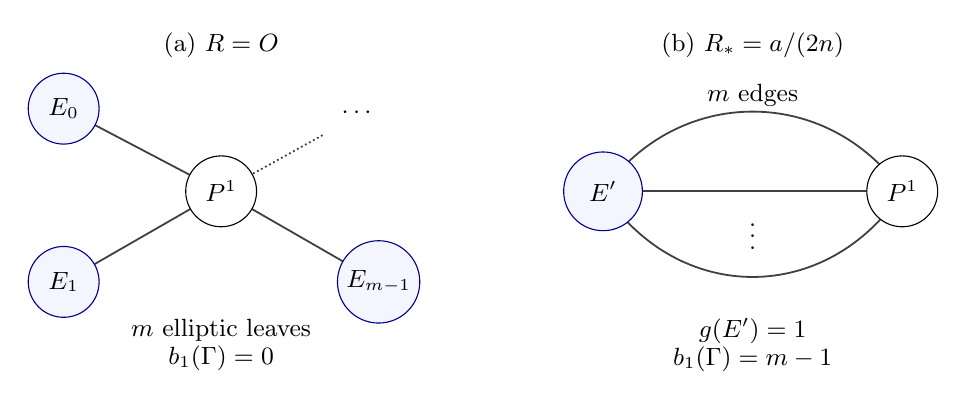
\begin{tikzpicture}[
  x=1cm,y=1cm,
  every node/.style={font=\small,inner sep=2pt},
  component/.style={draw,fill=white,circle,minimum size=9mm},
  elliptic/.style={component,draw=blue!55!black,fill=blue!4},
  edge/.style={draw=black!75,line width=.65pt}
]
  \node at (2.5,3.65) {\textup{(a)} $R=O$};
  \node at (9.25,3.65) {\textup{(b)} $R_*=a/(2n)$};

  \coordinate (rational) at (2.5,1.8);
  \coordinate (leafzero) at (.5,2.85);
  \coordinate (leafone) at (.5,.65);
  \coordinate (leaflast) at (4.5,.65);
  \draw[edge] (rational) -- (leafzero);
  \draw[edge] (rational) -- (leafone);
  \draw[edge] (rational) -- (leaflast);
  \draw[edge,densely dotted] (rational) -- (3.8,2.52);
  \node at (4.22,2.8) {$\cdots$};
  \node[component] at (rational) {$\mathbb P^1$};
  \node[elliptic] at (leafzero) {$E_0$};
  \node[elliptic] at (leafone) {$E_1$};
  \node[elliptic] at (leaflast) {$E_{m-1}$};
  \node[align=center] at (2.5,-.15)
    {$m$ elliptic leaves\\[-1pt] $b_1(\Gamma)=0$};

  \coordinate (emain) at (7.35,1.8);
  \coordinate (tail) at (11.15,1.8);
  \draw[edge] (emain) .. controls (8.3,3.15) and (10.2,3.15) .. (tail);
  \draw[edge] (emain) -- (tail);
  \draw[edge] (emain) .. controls (8.3,.35) and (10.2,.35) .. (tail);
  \node[fill=white,inner sep=1pt] at (9.25,1.33) {$\vdots$};
  \node[elliptic,minimum size=10mm] at (emain) {$E'$};
  \node[component] at (tail) {$\mathbb P^1$};
  \node at (9.25,3.02) {$m$ edges};
  \node[align=center] at (9.25,-.15)
    {$g(E')=1$\\[-1pt] $b_1(\Gamma)=m-1$};
\end{tikzpicture}

\caption{The dual graphs of the two special fibers.  Vertex labels
indicate component genera and identify the elliptic components; edges
are nodes.  At $R=O$ the graph is a star with $m$ elliptic leaves, so
the Jacobian is $E^m$.  At $R=a/(2n)$ two components meet in $m$
nodes, giving graph Betti number $m-1$.  The drawings are schematic
for general odd $m$.}
\label{geo:dual-graphs}
\end{figure}

The first degeneration has now supplied a split product fiber and a
neighborhood in which its homology can be compared with nearby smooth
fibers.  The second has supplied $m$ nodes, each with smoothing order
one.  We next identify their vanishing cycles in a single integral
basis.
